\documentclass{beamer}

\mode<presentation>


\usepackage{amsmath,amssymb,amsfonts,amsbsy,amsthm}
\usepackage{epsfig,array}
\usepackage[hidelinks]{hyperref}

\theoremstyle{plain}
\newtheorem{theorem}{Theorem}[section]
\newtheorem{algorithm}[theorem]{Algorithm}
\newtheorem{claim}[theorem]{Claim}
\newtheorem{conclusion}{Conclusion}
\newtheorem{condition}{Condition}
\newtheorem{conjecture}{Conjecture}
\newtheorem{corollary}[theorem]{Corollary}
\newtheorem{criterion}{Criterion}
\newtheorem{lemma}[theorem]{Lemma}
\newtheorem*{lemma*}{Lemma}
\newtheorem{prop}[theorem]{Proposition}

\theoremstyle{definition}
\newtheorem{definition}[theorem]{Definition}
\newtheorem{example}{Example}[section]
\newtheorem*{example*}{Example}
\newtheorem{exercise}[example]{Problem}
\newtheorem{problem}[example]{Problem}
\newtheorem{remark}[theorem]{Remark}
\newtheorem{ruleofthumb}[theorem]{Rule of thumb}
\newtheorem*{remark*}{Remark}
\newtheorem{reminder}[theorem]{Reminder}
%\newtheorem*{solution}{Solution}
\newtheorem{summary}{Summary}
%\newenvironment{proof}[1][Proof]{\textbf{#1.} }{\ \rule{0.5em}{0.5em}}
\newenvironment{solution}[1][{\bf Solution}]{ \emph{#1.} }{\medskip}
\newenvironment{notation}[1][\textbf{Notation:} ]{  #1}{\medskip}

\numberwithin{figure}{section}
\numberwithin{equation}{section}

% Definitions
%================================================================
\def\curl{{\rm curl}\,}
\def\div{{\rm div}\,}
\def\la{\lambda}
\def\ba{{\bf a}}
\def\bb{{\bf b}}
\def\be{{\bf e}}
\def\bj{{\bf j}}
\def\bn{{\bf n}}
\def\bV{{\bf V}}
\def\bJ{{\bf J}}
\def\bv{{\bf v}}
\def\bu{{\bf u}}
\def\bH{{\bf H}}
\def\vf{{\bf f}}
\def\bh{{\bf h}}
\def\bU{{\bf U}}
\def\bV{{\bf V}}
\def\bx{{\bf x}}
\def\by{{\bf y}}
\def\bz{{\bf z}}
\def\bX{{\bf X}}
\def\bC{{\bf C}}

\def\vx {{\bf x}}
\def\vy {{\bf y}}
\def\vz {{\bf z}}
\def\vv {{\bf v}}
\def\vV {{\bf V}}
\def\vu {{\bf u}}
\def\vb {{\bf b}}
\def\vc {{\bf c}}
\def\vr {{\bf r}}

\def\pr{{\partial}}
\def\eps{{\epsilon}}
\def\veta{\boldsymbol{\eta}}
\def\bxi{\boldsymbol{\xi}}
\def\bnu{\boldsymbol{\nu}}
\def\Bom{\boldsymbol{\Omega}}
\def\pd#1#2{\frac{\displaystyle\partial#1}{\displaystyle\partial#2}}
\def\bfr#1#2{\frac{\displaystyle #1}{\displaystyle #2}}
\def\vec#1{\boldsymbol{#1}}
\def\Bbb{\mathbb}
\def \shalf{{\textstyle \frac{1}{2}}}
\def \half{\frac{1}{2}}
\def \ssum{{\textstyle \sum}}



\begin{document}

\setbeamercovered{transparent}


%%%%%%%%%%%%%%%%%%%%%%%%%%%%%%%%%%%%%%%%%%%%%%%%%%%%%%%%%%%%%%%%%%%%%%%%%%%%%%%%%%%%%%%%%%%%%%%%%%%%%%%%%%%%%%%%%%%

\begin{frame}{Explicit finite-difference method for the heat equation}

\noindent
Consider the heat (diffusion) equation
\begin{equation}
u_{t} = K \, u_{xx}, \quad
0<x< L, \quad 0 < t < T,   \label{a1}
\end{equation}
subject to the boundary conditions
\begin{equation}
u(0, t) = u(L, t)=0 \quad \hbox{for} \quad t\in (0,T),   \label{a2}
\end{equation}
and initial condition
\begin{equation}
u(x, 0) = u_{0}(x),   \label{a3}
\end{equation}
where $u_{0}(x)$ is a given function. In Eq. (\ref{a1}), $K>0$.

\end{frame}

%%%%%%%%%%%%%%%%%%%%%%%%%%%%%%%%%%%%%%%%%%%%%%%%%%%%%%%%%%%%%%%%%%%%%%%%%%%%%%%%%%%%%%%%%%%%%%%%%%%%%%%%%%%%%%%%%%%


\begin{frame}{Grid points (or mesh points)}

Let $N,M\in\mathbb{N}$ and let
\[
\tau=\frac{T}{M}, \quad h=\frac{L}{N}.
\]
Then we define the grid points $(x_{k}, t_{j})$:
\begin{eqnarray}
&&x_{k}=hk \quad {\rm for} \quad k=0,1,\dots,N; \nonumber \\
&&t_{j}=\tau j \quad {\rm for} \quad j=0,1,\dots,M. \nonumber
\end{eqnarray}
The problem is to find numbers $w_{kj}$
such that $w_{kj}$ approximates the value of the exact solution
$u(x,t)$ at the grid point $(x_{k}, t_{j})$, i.e.
\[
w_{kj}\approx u(x_{k}, t_{j})
\]
for $k=0,1,\dots,N$ and $j=0,1,2,\dots$



\end{frame}

%%%%%%%%%%%%%%%%%%%%%%%%%%%%%%%%%%%%%%%%%%%%%%%%%%%%%%%%%%%%%%%%%%%%%%%%%%%%%%%%%%%%%%%%%%%%%%%%%%%%%%%%%%%%%%%%%%%


\begin{frame}{Grid points}

\begin{figure}[h]
\centering

\includegraphics[width=10cm,height=7cm]{../Lecture_notes/basic_grid2.pdf}
\end{figure}

\vskip 10mm

\end{frame}

%%%%%%%%%%%%%%%%%%%%%%%%%%%%%%%%%%%%%%%%%%%%%%%%%%%%%%%%%%%%%%%%%%%%%%%%%%%%%%%%%%%%%%%%%%%%%%%%%%%%%%%%%%%%%%%%%%%


\begin{frame}{Approximations to partial derivatives}

By definition,
\[
u_{t}(x_k,t_j)=\lim_{\tau\to 0}\frac{u(x_k,t_j+\tau)-u(x_k,t_j)}{\tau}.
\]
It is natural to expect that
\[
u_{t}(x_k,t_j)\approx \frac{u(x_k,t_j+\tau)-u(x_k,t_j)}{\tau}
\]
for sufficiently small $\tau$.

\vskip 5mm
\textcolor{blue}{What is the error of this formula?}

\end{frame}

%%%%%%%%%%%%%%%%%%%%%%%%%%%%%%%%%%%%%%%%%%%%%%%%%%%%%%%%%%%%%%%%%%%%%%%%%%%%%%%%%%%%%%%%%%%%%%%%%%%%%%%%%%%%%%%%%%%


\begin{frame}{Truncation error}

The first Taylor polynomial for $u(x_k,t_j+\tau)$:
\[
u(x_k,t_j+\tau)=u(x_k,t_j)+\tau \frac{\pr u}{\pr t}(x_k,t_j)+
\frac{\tau^2}{2}\frac{\pr^2 u}{\pr t^2}(x_k,\xi)
\]
where $\xi$ is between $t_j$ and $t_j+\tau$. Therefore,
\[
\tau_{kj}=\frac{\pr u}{\pr t}(x_k,t_j)-\frac{u(x_k,t_j+\tau)-u(x_k,t_j)}{\tau}=
-\frac{\tau}{2}\frac{\pr^2 u}{\pr t^2}(x_k,\xi).
\]
$\tau_{kj}$ is called the \textcolor{blue}{{\em truncation error }}.

\vskip 5mm
If $u_{tt}(x,t)$ is bounded, then
\[
\tau_{kj}=O(\tau) \quad {\rm as} \quad \tau\to 0.
\]

\end{frame}

%%%%%%%%%%%%%%%%%%%%%%%%%%%%%%%%%%%%%%%%%%%%%%%%%%%%%%%%%%%%%%%%%%%%%%%%%%%%%%%%%%%%%%%%%%%%%%%%%%%%%%%%%%%%%%%%%%%


\begin{frame}{Forward- and backward-difference formulae}
Formula
\[
u_{t}(x_k,t_j)\approx \frac{u(x_k,t_j+\tau)-u(x_k,t_j)}{\tau}
\]
for $\tau>0$ is called the {\bf forward-difference formula}.

\vskip 5mm
If we replace $\tau$ by $-\tau$, we obtain
the {\bf backward-difference formula}:
\[
u_{t}(x_k,t_j)\approx \frac{u(x_k,t_j)-u(x_k,t_j-\tau)}{\tau}.
\]


\end{frame}

%%%%%%%%%%%%%%%%%%%%%%%%%%%%%%%%%%%%%%%%%%%%%%%%%%%%%%%%%%%%%%%%%%%%%%%%%%%%%%%%%%%%%%%%%%%%%%%%%%%%%%%%%%%%%%%%%%%


\begin{frame}{Finite difference formula for $u_{xx}$}

From Taylor's theorem,
\begin{eqnarray}
u(x_k+h,t_j)&=&u(x_k,t_j)+h u_{x}(x_k,t_j)+
\frac{h^2}{2}u_{xx}(x_k,t_j) \nonumber \\
&&+
\frac{h^3}{6}u_{xxx}(x_k,t_{j})+
\frac{h^4}{24}u_{xxxx}(\xi_1,t_{j}), \nonumber \\
u(x_k-h,t_j)&=&u(x_k,t_j)-h u_{x}(x_k,t_j)+
\frac{h^2}{2}u_{xx}(x_k,t_j) \nonumber \\
&&-
\frac{h^3}{6}u_{xxx}(x_k,t_{j})+
\frac{h^4}{24}u_{xxxx}(\xi_2,t_{j}) \nonumber
\end{eqnarray}
for some $\xi_{1}$ between $x_{k}$ and $x_{k}+h$
and some $\xi_{2}$ between $x_{k}-h$ and $x_{k}$.

Now take the sum of these.

\end{frame}

%%%%%%%%%%%%%%%%%%%%%%%%%%%%%%%%%%%%%%%%%%%%%%%%%%%%%%%%%%%%%%%%%%%%%%%%%%%%%%%%%%%%%%%%%%%%%%%%%%%%%%%%%%%%%%%%%%%


\begin{frame}{}
The sum of these yields
\begin{eqnarray}
u(x_k+h,t_j)+u(x_k-h,t_j)&=&2u(x_k,t_j)+ h^2u_{xx}(x_k,t_j) \nonumber \\
&&+ \frac{h^4}{24}\left[u_{xxxx}(\xi_1,t_{j}) +
u_{xxxx}(\xi_2,t_{j})\right].  \nonumber
\end{eqnarray}
The number
\[
\frac{1}{2}\left[u_{xxxx}(\xi_{1}, t_{j})+u_{xxxx}(\xi_{2},t_{j})\right]
\]
is between
\[
u_{xxxx}(\xi_{1},t_{j}) \quad {\rm and} \quad u_{xxxx}(\xi_{2},t_{j}).
\]
If $u_{xxxx}$ is continuous, then
by the intermediate value theorem,
\[
\frac{1}{2}\left[u_{xxxx}(\xi_{1},t_{j})+u_{xxxx}(\xi_{2},t_{j})\right]
=u_{xxxx}(\xi,t_{j}).
\]
for some $\xi$ between $\xi_{1}$ and $\xi_{2}$.





\end{frame}

%%%%%%%%%%%%%%%%%%%%%%%%%%%%%%%%%%%%%%%%%%%%%%%%%%%%%%%%%%%%%%%%%%%%%%%%%%%%%%%%%%%%%%%%%%%%%%%%%%%%%%%%%%%%%%%%%%%


\begin{frame}{}
Hence,
\[
u_{xx}(x_k,t_j)=\frac{u(x_{k+1},t_j)-2u(x_k,t_j)+u(x_{k-1},t_j)}{h^2}
-\frac{h^2}{12}u_{xxxx}(\xi,t_{j}),
\]
where $\xi\in(x_{k-1},x_{k+1})$.

This is called the {\bf central difference formula} for $u_{xx}$.
If $u_{xxxx}$ is bounded, the truncation error is $O(h^2)$


\end{frame}

%%%%%%%%%%%%%%%%%%%%%%%%%%%%%%%%%%%%%%%%%%%%%%%%%%%%%%%%%%%%%%%%%%%%%%%%%%%%%%%%%%%%%%%%%%%%%%%%%%%%%%%%%%%%%%%%%%%


\begin{frame}{Forward-difference method for the heat eqn.}

Let
\[
w_{kj}\approx u(x_{k},t_{j}).
\]
Then
\[
\frac{w_{k,j+1}-w_{kj}}{\tau}-K
\frac{w_{k+1, j}-2w_{kj}+w_{k-1,j}}{h^{2}}=0,
\]
for each interior grid point. Local truncation error is $O(\tau)$+$O(h^2)$.

{\bf Boundary conditions:}
\[
w_{0,j}=w_{N,j}=0  \quad
{\rm for \ each} \ \ j=1, \dots, M.
\]
{\bf Initial conditions:}
\[
w_{k,0}=u_{0}(x_{k})  \quad
{\rm for \ each} \ \ k=0, 1, \dots, N.
\]


\end{frame}

%%%%%%%%%%%%%%%%%%%%%%%%%%%%%%%%%%%%%%%%%%%%%%%%%%%%%%%%%%%%%%%%%%%%%%%%%%%%%%%%%%%%%%%%%%%%%%%%%%%%%%%%%%%%%%%%%%%


\begin{frame}{\small Matrix form}

{\small
The equivalent difference equation
\[
w_{k,j+1}=\left(1-2\gamma\right)w_{kj}+
\gamma\left(
w_{k+1, j}+w_{k-1,j}\right), \quad \gamma\equiv \frac{K\tau}{h^{2}}.
\]
can be written as
\[
{\bf w}^{(j)}=A{\bf w}^{(j-1)} \quad \hbox{for} \quad j=1,2,\dots,
\]
where
\[
A=\left[
\begin{array}{cccccc}
1-2\gamma &\gamma &0      &\dots  &\dots &0 \\
\gamma &1-2\gamma &\gamma &\ddots  &     &\vdots \\
0      &\gamma &1-2\gamma &\gamma &\ddots &\vdots \\
\vdots &\ddots &\ddots &\ddots &\ddots &0 \\
\vdots &       &\ddots &\ddots &\ddots &\gamma \\
0      &\dots  &\dots  &0      &\gamma &1-2\gamma
\end{array}\right], \quad
{\bf w}^{(j)}=\left[
\begin{array}{c}
w_{1,j} \\
w_{2,j} \\
\vdots \\
\vdots \\
\vdots \\
w_{N-1,j}
\end{array}\right].
\label{b7}
\]
The forward-difference method is an example of an {\bf explicit finite-difference method}.
}

\end{frame}

%%%%%%%%%%%%%%%%%%%%%%%%%%%%%%%%%%%%%%%%%%%%%%%%%%%%%%%%%%%%%%%%%%%%%%%%%%%%%%%%%%%%%%%%%%%%%%%%%%%%%%%%%%%%%%%%%%%


\begin{frame}{Example}

{\small
Let's employ the forward-difference method to solve the heat equation
\[
u_{t}=u_{xx} \quad \textrm{for} \quad 0<x<1  \quad \textrm{and} \quad 0<t<0.1
\]
subject to zero boundary conditions
\[
u(0,t)=0, \quad u(1,t)=0
\]
and the initial condition
\[
u(x,0)=2\sin(2\pi x).
\]

\vskip 5mm
Note that the \textbf{exact} solution is given by
\[
u(x,t)=2e^{-4\pi^2 t}\sin(2\pi x).
\]

}
\end{frame}
%%%%%%%%%%%%%%%%%%%%%%%%%%%%%%%%%%%%%%%%%%%%%%%%%%%%%%%%%%%%%%%%%%%%%%%%%%%%%%%%%%%%%%%

\begin{frame}{Stability}

{\small Let ${\bf w}^{(j)}$ be the solution generated by the formula
\[
{\bf w}^{(j)}=A{\bf w}^{(j-1)}
\]
from the initial data ${\bf w}^{(0)}$.

\vskip 3mm

Let $\tilde{\bf w}^{(j)}$ be the solution generated by the same formula from slightly different
initial data
\[
\tilde{\bf w}^{(0)}={\bf w}^{(0)}+{\bf z}^{(0)}
\]
where ${\bf z}^{(0)}$ is the initial error (perturbation).

\vskip 3mm

\textit{If the errors grow with each time step, then the
difference method in \textbf{unstable}. If they do not grow, it is stable.}

\vskip 3mm

\textcolor{blue}{How to find out whether the forward-difference method is stable?}
}

\end{frame}

%%%%%%%%%%%%%%%%%%%%%%%%%%%%%%%%%%%%%%%%%%%%%%%%%%%%%%%%%%%%%%%%%%%%%%%%%%%%%%%%%%%%%%%%%%%%%%%%%%%%%%%%%%%%%%%%%%%


\begin{frame}{Example: stable scheme}
\begin{figure}[h]
\centering
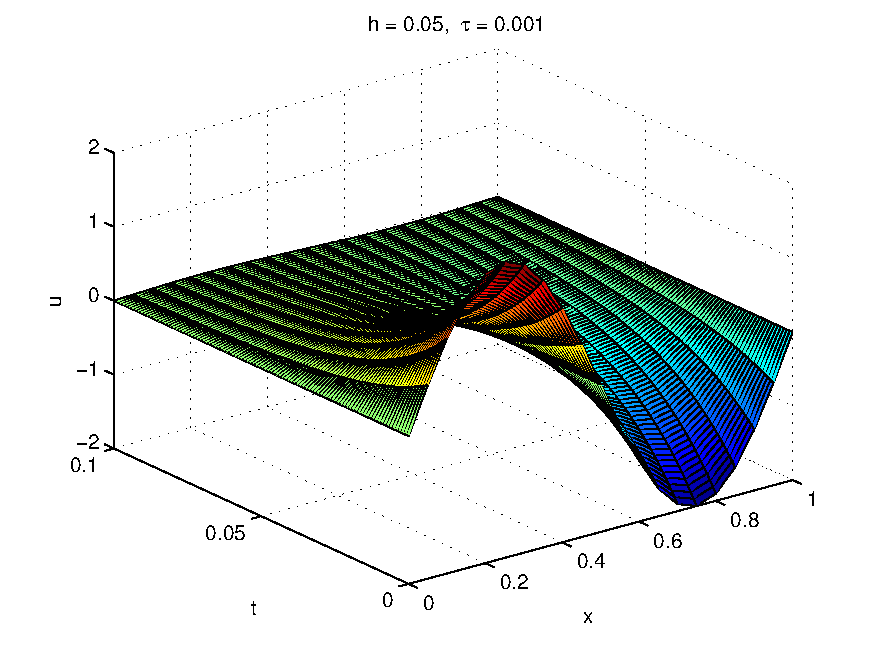
\includegraphics[width=10cm,height=7cm]{../Lecture_notes/forward_diff_fig1.pdf}
\end{figure}


\end{frame}

%%%%%%%%%%%%%%%%%%%%%%%%%%%%%%%%%%%%%%%%%%%%%%%%%%%%%%%%%%%%%%%%%%%%%%%%%%%%%%%%%%%%%%%%%%%%%%%%%%%%%%%%%%%%%%%%%%%


\begin{frame}{Example: unstable scheme}
\begin{figure}[h]
\centering
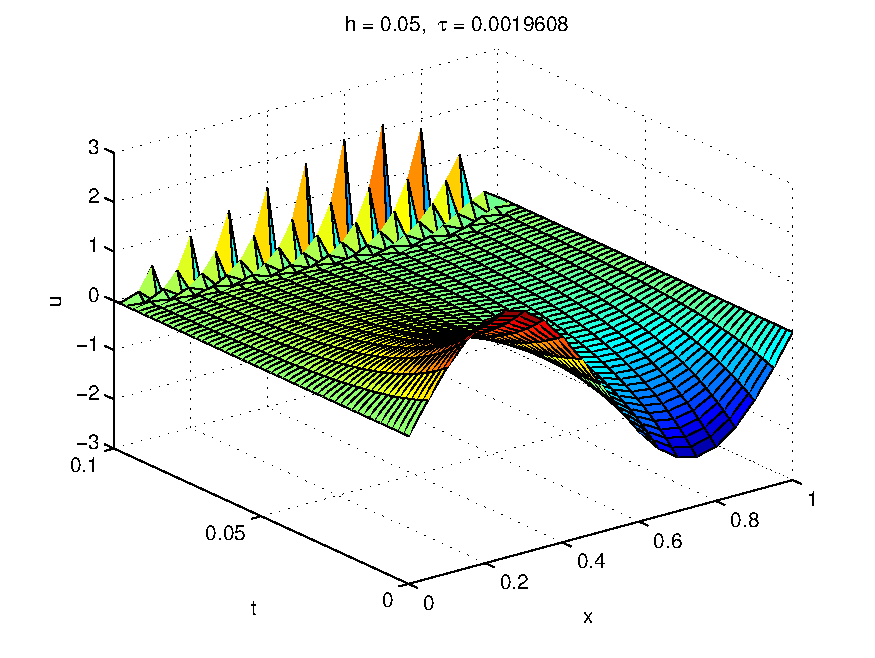
\includegraphics[width=10cm,height=7cm]{../Lecture_notes/forward_diff_fig2.pdf}
\end{figure}


\end{frame}
%%%%%%%%%%%%%%%%%%%%%%%%%%%%%%%%%%%%%%%%%%%%%%%%%%%%%%%%%%%%%%%%%%%%%%%%%%%%%%%%%%%%%%%%%%%%%%%%%%%%%%%%%%%%%%%%%%%

\begin{frame}{Stability}

{\small

\textbf{Matrix method.}

\begin{itemize}

\item We have
\[
\tilde{\bf w}^{(1)}=A\tilde{\bf w}^{(0)}=A\left({\bf w}^{(0)}+{\bf z}^{(0)}\right)=A{\bf w}^{(0)}+A{\bf z}^{(0)},
\]
i.e.
\[
{\bf z}^{(1)}=\tilde{\bf w}^{(1)}-{\bf w}^{(1)}=A{\bf z}^{(0)}.
\]
\item At the $n$-th time step,
\[
{\bf z}^{(n)}=\tilde{\bf w}^{(n)}-{\bf w}^{(n)}=A^n{\bf z}^{(0)}.
\]
\item The method is stable if
for any initial error ${\bf z}^{(0)}$,
\[
\Vert A{\bf z}^{(0)}\Vert\leq \Vert {\bf z}^{(0)}\Vert
\]
Here $\Vert\cdot\Vert$ is any vector norm.

\item This is
equivalent to
\[
\vert\lambda_{i}\vert\leq 1 \quad \hbox{for} \quad i=1, 2, \dots, N-1,
\]
where the $\lambda_i$ are the eigenvalues of matrix $A$.

\end{itemize}
}

\end{frame}

%%%%%%%%%%%%%%%%%%%%%%%%%%%%%%%%%%%%%%%%%%%%%%%%%%%%%%%%%%%%%%%%%%%%%%%%%%%%%%%%%%%%%%%%%%%%%%%%%%%%%%%%%%%%%%%%%%%


\begin{frame}{\small Periodic boundary conditions}

{\small
If we impose $u(x,0)=u(x,L)$ then $w_N = w_0$. We also define
$w_{N+1}=w_{1}$ Then we can use forward difference
equation
\[
w_{k,j+1}=\left(1-2\gamma\right)w_{kj}+
\gamma\left(
w_{k+1, j}+w_{k-1,j}\right)
\]
for $k=1,\dots N$. Which can be written as
${\bf w}^{(j)}=A{\bf w}^{(j-1)} $
where now
\[
A=\left[
\begin{array}{cccccc}
1-2\gamma &\gamma &0      &\dots  &0 &\gamma \\
\gamma &1-2\gamma &\gamma &\ddots  &\vdots &0\\
0      &\gamma &1-2\gamma &\gamma &\ddots &\vdots \\
\vdots &\ddots &\ddots &\ddots &\ddots &0 \\
0 &       &\ddots &\ddots &\ddots &\gamma \\
\gamma      &0  &\dots  &0      &\gamma &1-2\gamma
\end{array}\right], \quad
{\bf w}^{(j)}=\left[
\begin{array}{c}
w_{1,j} \\
w_{2,j} \\
\vdots \\
\vdots \\
\vdots \\
w_{N,j}
\end{array}\right].
\label{bp7}
\]
}
This is a circulant matrix and its eigenvectors are known.
\end{frame}


%%%%%%%%%%%%%%%%%%%%%%%%%%%%%%%%%%%%%%%%%%%%%%%%%%%%%%%%%%%%%%%%%%%%%%%%%%%%%%%%%%%%%%%%%%%%%%%%%%%%%%%%%%%%%%%%%%%

\begin{frame}{Stability}

{\small

\textbf{Fourier method.}


Let $w_{kj}$  and $\tilde{w}_{kj}$ be two solutions of the difference equation
\[
\frac{w_{k,j+1}-w_{k,j}}{\tau}-K\frac{w_{k+1,j}-2w_{k,j}+w_{k-1,j}}{h^2}=0,
\]
corresponding to slightly different initial data.
Then the error (perturbation) $z_{kj}=\tilde{w}_{kj}-w_{kj}$ satisfies the equation
\[
\frac{z_{k,j+1}-z_{k,j}}{\tau}-K\frac{z_{k+1,j}-2z_{k,j}+z_{k-1,j}}{h^2}=0.
\]
We seek a particular solution of this equation in the form
\[
z_{k,j}=\rho_{q}^{j}e^{iqx_{k}}, \quad q\in{\mathbb R}.
\]
\textbf{The finite-difference method
is stable, if all solutions having this form are such that}
\[
\vert\rho_{q}\vert\leq 1 \quad {\rm for \ all} \ \ q\in{\mathbb R}.
\]
}

\end{frame}

%%%%%%%%%%%%%%%%%%%%%%%%%%%%%%%%%%%%%%%%%%%%%%%%%%%%%%%%%%%%%%%%%%%%%%%%%%%%%%%%%%%%%%%%%%%%%%%%%%%%%%%%%%%%%%%%%%%

\begin{frame}{Stability}
Substituting $z_{k,j}=\rho_{q}^{j}e^{iqx_{k}}$ gives
\[
\frac{\rho_{q}^{j+1}e^{iqx_{k}}-\rho_{q}^{j}e^{iqx_{k}}}{\tau}-
K\frac{\rho_{q}^{j}\left(e^{iqx_{k+1}}-2e^{iqx_{k}}+e^{iqx_{k-1}}\right)}{h^2}=0
\]
or
\[
\rho_{q}-1 - \gamma \left(e^{iqh}-2+e^{-iqh}\right)=0.
\]
Since
\[
e^{iqh}-2+e^{-iqh}=\left(e^{iqh/2}-e^{-iqh/2}\right)^{2}=-4\sin^{2}
\frac{qh}{2},
\]
we obtain
\[
\rho_{q}=1-4\gamma\sin^{2} \frac{qh}{2}.
\]
The method is stable if
\[
-1\leq 1-4\gamma\sin^{2}\frac{qh}{2}\leq 1 .
\]



\end{frame}

%%%%%%%%%%%%%%%%%%%%%%%%%%%%%%%%%%%%%%%%%%%%%%%%%%%%%%%%%%%%%%%%%%%%%%%%%%%%%%%%%%%%%%%%%%%%%%%%%%%%%%%%%%%%%%%%%%%

\begin{frame}{Stability}
The stability condition is equivalent to
\[
0\leq \gamma\sin^{2}\frac{qh}{2}\leq \frac{1}{2},
\]
for all $q$, which means that
\[
0\leq\gamma \leq \frac{1}{2} \quad \text{ or equivalently} \quad0\leq \tau \leq
\frac{h^2}{2K}. 
\]

\vskip 3mm   A method which is stable only if a certain
condition holds is called {\bf conditionally stable}. 

The
forward-difference method for the heat equation is conditionally
stable.

\end{frame}


\end{document}
